\documentclass[11pt]{article}
\usepackage{listings}
\usepackage{tikz}
\usepackage{enumerate}
\usepackage{url}
\usepackage{amssymb}
\usetikzlibrary{arrows,automata,shapes}

\lstset{basicstyle=\ttfamily \scriptsize,
  basicstyle=\ttfamily,
   columns=fullflexible,
   breaklines=true,
   numbers=left,
   numberstyle=\scriptsize,
   stepnumber=1,
   mathescape=false,
   tabsize=2,
   showstringspaces=false
}
\newtheorem{defn}{Definition}
\newtheorem{crit}{Criterion}

\newcommand{\handout}[5]{
  \noindent
  \begin{center}
  \framebox{
    \vbox{
      \hbox to 5.78in { {\bf Software Testing, Quality Assurance and Maintenance } \hfill #2 }
      \vspace{4mm}
      \hbox to 5.78in { {\Large \hfill #5  \hfill} }
      \vspace{2mm}
      \hbox to 5.78in { {\em #3 \hfill #4} }
    }
  }
  \end{center}
  \vspace*{4mm}
}

\newcommand{\lecture}[4]{\handout{#1}{#2}{#3}{#4}{Lecture #1}}
% 1-inch margins, from fullpage.sty by H.Partl, Version 2, Dec. 15, 1988.
\topmargin 0pt
\advance \topmargin by -\headheight
\advance \topmargin by -\headsep
\textheight 8.9in
\oddsidemargin 0pt
\evensidemargin \oddsidemargin
\marginparwidth 0.5in
\textwidth 6.5in

\parindent 0in
\parskip 1.5ex
%\renewcommand{\baselinestretch}{1.25}

% http://gurmeet.net/2008/09/20/latex-tips-n-tricks-for-conference-papers/
\newcommand{\squishlist}{
 \begin{list}{$\bullet$}
  { \setlength{\itemsep}{0pt}
     \setlength{\parsep}{3pt}
     \setlength{\topsep}{3pt}
     \setlength{\partopsep}{0pt}
     \setlength{\leftmargin}{1.5em}
     \setlength{\labelwidth}{1em}
     \setlength{\labelsep}{0.5em} } }
\newcommand{\squishlisttwo}{
 \begin{list}{$\bullet$}
  { \setlength{\itemsep}{0pt}
     \setlength{\parsep}{0pt}
    \setlength{\topsep}{0pt}
    \setlength{\partopsep}{0pt}
    \setlength{\leftmargin}{2em}
    \setlength{\labelwidth}{1.5em}
    \setlength{\labelsep}{0.5em} } }
\newcommand{\squishend}{
  \end{list}  }

\lstdefinelanguage{JavaScript}{
  keywords={typeof, new, true, false, catch, function, return, null, catch, switch, var, if, in, while, do, else, case, break},
  keywordstyle=\color{blue}\bfseries,
  ndkeywords={class, export, boolean, throw, implements, import, this},
  ndkeywordstyle=\color{darkgray}\bfseries,
  identifierstyle=\color{black},
  sensitive=false,
  comment=[l]{//},
  morecomment=[s]{/*}{*/},
  commentstyle=\color{purple}\ttfamily,
  stringstyle=\color{red}\ttfamily,
  morestring=[b]',
  morestring=[b]''
}


\begin{document}

\lecture{11 --- January 28, 2015}{Winter 2015}{Patrick Lam}{version 1}

Assertions are a key ingredient in writing tests, so I thought I would
explicitly describe them.

\begin{defn}
  An \emph{assertion} contains an expression that is
  supposed to evaluate to {\tt true}.
\end{defn}

For instance, if we have a linked list, then the doubly-linked list
property states that {\tt prev} is the inverse of {\tt next}, i.e. for
nodes {\tt n}, we have {\tt n.next.prev == n}. After inserting a node,
one might expect this property to be true of that node (possibly with
caveats, for instance about the end of the list.)

  \begin{center}
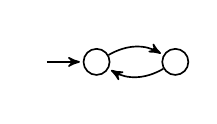
\begin{tikzpicture}[->,>=stealth',shorten >=1pt,auto,node distance=1cm,
                    semithick,initial text=]

  \node[circle,draw,initial]   (0)                    {};
  \node[circle,draw]   (1) [right of=0]  {};
  
  \path (0) edge [bend left]  node {} (1)
        (1) edge [bend left]  node {} (0);
\end{tikzpicture}
  \end{center}

We use assertions in unit tests to say what's supposed to be true.
  
\paragraph{Preconditions and postconditions.}
More generally, we can express
  what is supposed to be true upon entry \& exit from a method.

We saw this code in Linux:
  \begin{lstlisting}
/* LOCKING: caller. */
void ata_dev_select(...) { ...}
  \end{lstlisting}
This expresses an assertion (although not written as a program statement) that the lock is held upon entry.
  
\paragraph{Assume/Guarantee Reasoning.} 
Why would you use preconditions and postconditions? Reasoning about programs is difficult,
and preconditions and postconditions simplifies reasoning.

  When reasoning about the callee, you get to assume that the precondition holds upon entry.

  When reasoning about the caller, you get to guarantee the precondition holds before the call.

  The reverse holds about the postcondition.

\subsection*{aComment}
We talked about the aComment approach for locking-related annotations.
In particular, it:
\squishlist
\item extracts locking-related annotations from code;
\item extracts locking-related annotations from comments; and
\item propagates annotations to callers.
  \squishend

\subsection*{Tools}

To provide some context, consider the OS X Mavericks goto fail bug:

{ \scriptsize
\begin{lstlisting}[language=C]
  if ((err = SSLHashSHA1.update(&hashCtx, &serverRandom)) != 0)
      goto fail;
  if ((err = SSLHashSHA1.update(&hashCtx, &signedParams)) != 0)
      goto fail;
      goto fail;  /* MISTAKE! THIS LINE SHOULD NOT BE HERE */
  if ((err = SSLHashSHA1.final(&hashCtx, &hashOut)) != 0)
      goto fail;
      err = sslRawVerify(...);

  fail:
      return err;
\end{lstlisting}
}

The bug:\\
{\scriptsize \url{opensource.apple.com/source/Security/Security-55471/libsecurity_ssl/lib/sslKeyExchange.c} }

No bug:\\
{\scriptsize \url{www.opensource.apple.com/source/Security/Security-55179.13/libsecurity_ssl/lib/sslKeyExchange.c} }

A writeup:\\ {\scriptsize \url{nakedsecurity.sophos.com/2014/02/24/anatomy-of-a-goto-fail-apples-ssl-bug-explained-plus-an-unofficial-patch/}}

\paragraph{Detecting goto fail.}
In retrospect, a number of tools could've found this bug:
\squishlist
    \item compiler {\tt -Wunreachable-code} option
    \item PC-Lint:warning 539: Did not expect positive indentation
    \item PVS-Studio:V640: Logic does not match formatting
\squishend
The problem is that these tools also report many other issues, and live issues can be
buried among those other issues.

\subsection*{The Landscape of Testing and Static Analysis Tools}
Here's a survey of your options:
\squishlist
    \item manual testing;
    \item running a JUnit test suite, manually generated;
    \item running automatically-generated tests;
    \item running static analysis tools.
\squishend
We'll examine several points on this continuum today.
More on this later (Lecture 23), thanks to guest lecturer. Some examples:
\squishlist
    \item Coverity: a static analysis tool used by 900+ companies, 
      including BlackBerry, Mozilla, etc.
    \item Microsoft requires Windows device drivers 
      to pass their Static Driver Verifier for certification.
\squishend
      
\subsection*{Tools for Java that you can download}

\paragraph{FindBugs.} An open-source static bytecode analyzer for Java out of
the University of Maryland.
\begin{center}
  \url{findbugs.sourceforge.net}
\end{center}
It finds bug patterns:
\squishlist
    \item off-by-one;
    \item null pointer dereference;
    \item ignored {\tt read()} return value;
    \item ignored return value (immutable classes);
    \item uninitialized read in constructor;
    \item and more\ldots
\squishend

FindBugs gives some false positives. 
Here are some techniques to help avoid them:
\begin{center}
  \url{patricklam.ca/papers/14.msr.saa.pdf}
\end{center}

\paragraph{Java Path Finder (JPF), NASA.}
The key idea:
Implement a Java Virtual Machine,
    but explore many thread interleavings,
    looking for concurrency bugs.

\begin{center}    
  ``JPF is an explicit state software model checker for Java\texttrademark ~bytecode.''
\end{center}

JPF can also search for deadlocks and unhandled exceptions ({\tt NullPointerException}, {\tt AssertionError}); race conditions; missing heap bounds checks; and more.

\begin{center}
  \url{javapathfinder.sourceforge.net}
\end{center}

\paragraph{Korat (University of Illinois).}
Key Idea: Generate Java objects from a representation invariant specification
written as a Java method.

For instance, here's a binary tree.
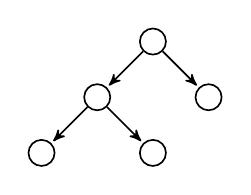
\begin{tikzpicture}[->,>=stealth',shorten >=1pt,auto,node distance=1cm,
                    semithick,initial text=]

  \node[circle,draw]   (0)                    {};
  \node[circle,draw]   (1) [below left of=0]  {};
  \node[circle,draw]   (2) [below right of=0] {};
  \node[circle,draw]   (3) [below left of=1] {};
  \node[circle,draw]   (4) [below right of=1] {};
  
  \path (0) edge              node {} (1)
        (0) edge              node {} (2)
        (1) edge              node {} (3)
        (1) edge              node {} (4);
\end{tikzpicture} \hspace*{2em} Binary Tree!\\[1em]

One characteristic of a binary tree:
\begin{itemize}
\item left \& right pointers don't refer to same node.
\end{itemize}

\newpage We can express that characteristic in Java as follows:
\begin{lstlisting}[language=Java]
boolean repOk() {
  if (root == null) return size == 0; 	   	      // empty tree has size 0
  Set visited = new HashSet(); visited.add(root);
  List workList = new LinkedList(); workList.add(root);
  while (!workList.isEmpty()) {
    Node current = (Node)workList.removeFirst();
    if (current.left != null) {
      if (!visited.add(current.left)) return false; // acyclicity
      workList.add(current.left);
    }
    if (current.right != null) {
      if (!visited.add(current.right)) return false; // acyclicity
      workList.add(current.right);
    }
  }
  if (visited.size() != size) return false; 	     // consistency of size
  return true;
}
\end{lstlisting}

Korat then generates all distinct (``non-isomorphic'') trees, 
    up to a given size (say 3).
It uses these trees as inputs for testing 
    the {\tt add()} method of the tree (or for any other methods.)

    \begin{center}
    \url{korat.sourceforge.net/index.html}
  \end{center}

    \paragraph{Randoop (MIT).}
    Key Idea:
    ``Writing tests is a difficult and time-consuming activity, 
  and yet it is a crucial part of good software engineering. 
  Randoop automatically generates unit tests for Java classes.''

  Randoop generates random sequence of method calls, 
  looking for object contract violations.
  
  To use it, simply point it at a program \& let it run.

  Randoop discards bad method sequences 
(e.g. illegal argument exceptions). It remembers method sequences that create complex objects,
    and sequences that result in object contract violations.\

  \begin{center}
    \url{code.google.com/p/randoop/}
  \end{center}

  Here is an example generated by Randoop:
  {\scriptsize
\begin{lstlisting}[language=Java]
public static void test1() {
    LinkedList list = new LinkedList();
    Object o1 = new Object();
    list.addFirst(o1);

    TreeSet t1 = new TreeSet(list);
    Set s1 = Collections.synchronizedSet(t1);

    // violated in the Java standard library!
    Assert.assertTrue(s1.equals(s1));
  }
\end{lstlisting}
}

\end{document}
